\chapter{Badanie wydajności}
\section{Baza sprzętowa}
\par{
Przy użyciu darmowego darmowego narzędzia ustalono następującą konfigurację sprzętowo-programową dostępną dla systemu operacyjnego.
\begin{itemize}
\item Procesor --- \textit{2x Intel(R) Core(TM)2 Duo CPU P8400 @ 2.26GHz}
\item Pamieć RAM --- \textit{4063MB DDR2 8000MHz}
\item System operacyjny --- \textit{Debian GNU/Linux jessie/sid}
\item Wersja jądra systemu --- \textit{3.2.0-4}
\item Dysk twardy --- \textit{500GB, 5400 rpm}
\item Wykorzystany system plików --- \textit{ext4}
\end{itemize}
}

\section{Plan badań}
\par{
Zaplanowane badanie miało za zadanie potwierdzić lub zaprzeczyć hipotezie, że kluczowe z punktu widzenia wydajności całej symulacji są czasy operacji wejścia-wyjścia nie zaś czasy obliczeń.
}
\par{
Aby sprawdzić tę teorię postanowiono przebadać czasy pojedynczego obiegu pętli symulacji w zależności od liczby obiektów symulowanych, przy stałej architekturze symulowanego miasta, stałym pokryciu czujnikami dla włączonego zapisu do bazy (standardowa wersja aplikacji) oraz dla operacji zapisu do bazy zastąpionej programową zaślepką nie wykonującą dodatkowych operacji.
}
\par{
Wartości wyżej wspomnianych stałych pokazuje tablica \ref{cost_table}.
}
\begin{table}[t]
\caption{Parametry symulacji użyte w badaniach}
\label{cost_table}
\begin{center}
\begin{tabular}{|c|c|}
  \hline 
  \textbf{Parametr} & \textbf{Wartość} \\
  \hline
  Minimalny czas obiegu pętli & \textit{32ms} \\
  Pokrycie czujnikami & \textit{66.(6)\%} \\
  Ilość obiegów pętli do średniej & \textit{1000} \\
  \hline  
\end{tabular}
\end{center}
\end{table}

\subsection{Czas pętli a ilość zapisów}
\par{
Przy planowaniu badań zauważono, że jeśli postawiona hipoteza była by prawdziwa, to kluczowe z punktu widzenia badanego czasu pojedynczego obiegu pętli była by ilość odczytów jakie czyniły czujniki w czasie takiego obiegu. Z tego względu zdecydowano się w ramach planowania właściwego eksperymentu na zbadanie zależności między liczbą obiektów w symulacji a czasem obiegu pojedynczej symulacji. Efekt tej pracy przedstawia tablica \ref{ex_1} oraz wykres \ref{ex_1_chart}.
}
\par{
\begin{table}[t]
\caption{Zależność czasu trwania pętli od liczby obiektów}
\label{ex_1}
\begin{center}
\begin{tabular}{|c|c|}
  \hline 
 \textbf{Liczba obiektów} & \textbf{Czas trwania pętli (ms)} \\
  \hline
  10 & 3,5 \\
  20	 & 5 \\
  40	 & 12 \\
  60	 & 18 \\
  80	 & 26 \\
  100 & 35 \\
  150 & 2413 \\
  200 & 3041 \\
  300 & 4292 \\
  400 & 6553 \\
  \hline  
\end{tabular}
\end{center}
\end{table}
}

\begin{figure}[!ht]
    \begin{center}
	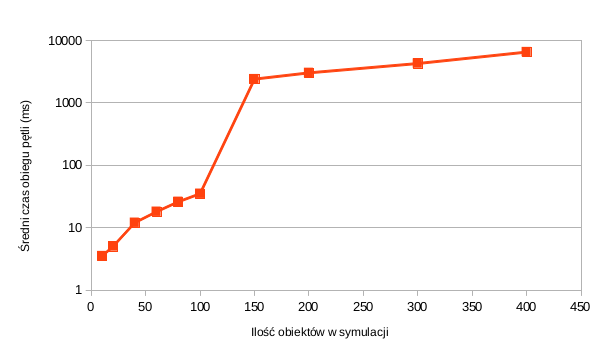
\includegraphics[width=\textwidth,keepaspectratio]{img/wykres_1}
	\caption{Liczba obiektów a średni czas obiegu pętli.}
	\label{ex_1_chart}
    \end{center}
\end{figure}

\par{
Na wykresie wyraźnie widać, zależność liczby zapisów od ilości obiektów ma charakter liniowy w dwóch przedziałach z wyraźnym przesunięciem w okolicach 120 obiektów. Powodem tego załamania zdaje się być fakt przekroczenia przez czas jednego obiegu pętli zadanego jako stała minimalnego czasu przetwarzania.  Powoduje to, że kolejny obieg pętli będzie odpowiadał dłuższemu odcinkowi symulowanego czasu a więc średnio będzie nań przypadało więcej odczytów z kamer (jako, że kamera odczytuje stan okolicy periodycznie). Zależnie od prawdziwości wyżej wspomnianej hipotezy powinna nastąpić w tym miejscu mniej lub bardziej gwałtowna reakcja lawinowa prowadząca do stanu, w którym każda kamera będzie dokonywała odczytu w każdym obiegu pętli --- to właśnie obserwujemy jako załamanie na rysunku \ref{ex_1_chart}.
}
\par{
Ze względu na dualny charakter tej charakterystyki zdecydowano się przenieść ją do celów badań do jej górnej części, by to załamanie --- nieistotne z punktu widzenia celu badan --- nie zaciemniało obrazu. W związku z tym zdecydowano się obniżyć czas między wyzwoleniami każdej z kamer do zera co powoduje, że każda kamera w każdym obiegu pętli wykona zrzut swojego otoczenia, ponieważ spełniony będzie warunek:
}
\par{
\begin{center}
$\Delta T_{wyzwolenia kamer} < \Delta T_{kroku}$
\end{center}
}

\section{Wyniki badań}
\par{
W wyniku badań otrzymano rezultaty zaprezentowane w tablicy \ref{ex_2} oraz na wykresie \ref{ex_2_chart}.
}

\par{
\begin{table}[t]
\caption{Liczba obiektów a średni czas pętli, dla $\Delta T_{wyzwolenia kamer} = 0$}
\label{ex_2}
\begin{center}
\begin{tabular}{|c|c|c|}
  \hline 
  \textbf{Liczba obiektów} & \textbf{$T_{petli, zapis do bazy} (ms)$} & \textbf{$T_{petli, zapis do bazy wylaczony} (ms)$}\\
  \hline
10 & 177 & 2 \\
20 & 375 & 2,5 \\
40 & 674 & 3 \\
80 & 1222 & 4 \\
160 & 2629 & 7 \\
320 & 5052 & 13 \\
640 & 10028 & 31 \\
  \hline  
\end{tabular}
\end{center}
\end{table}
}

\begin{figure}[!ht]
    \begin{center}
	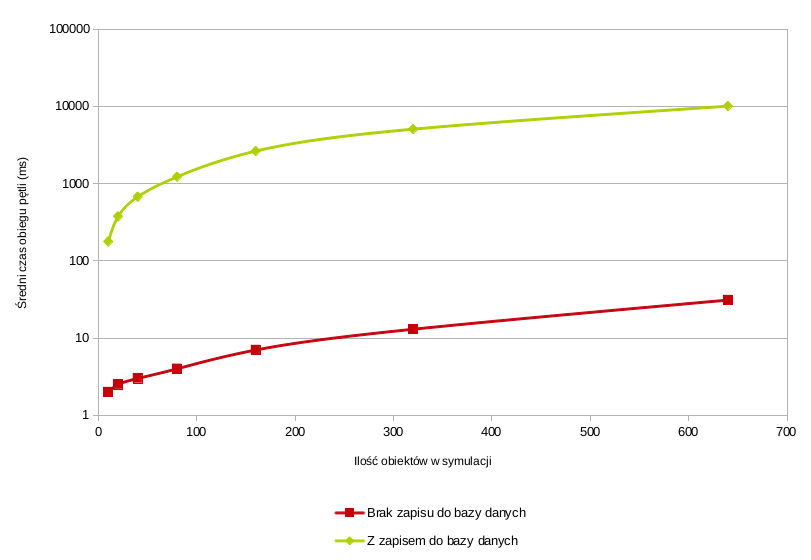
\includegraphics[width=\textwidth,keepaspectratio]{img/wykres_2}
	\caption{Liczba obiektów a średni czas obiegu pętli dla $\Delta T_{wyzwolenia kamer} = 0$.}
	\label{ex_2_chart}
    \end{center}
\end{figure}


\par{
Na wykresie \ref{ex_2_chart} (skala logarytmiczna) wyraźnie widać, że zarówno w przypadku zapisu do bazy danych jak i gdy zapis ten zostanie wyłączony czas trwania pojedynczego obiegu pętli zależy liniowo od ilości obiektów w symulacji.
}
\par{
Na wykresie w skali logarytmicznej widać też jednak, że w przypadku zapisów do bazy cały wykres przeniesiony jest o rzędy wielkości wyżej - na wykresie w zwykłej skali wariant bez zapisu byłby w ogóle nie widoczny i zredukowany do płaskiego odcinka na dole wykresu.
}
\par{
Wnioskiem z tej obserwacji zdaje się być potwierdzenie hipotezy, że kluczowym elementem z punktu widzenia wydajności projektowanej aplikacji jest wydajność bazy danych natomiast wydajność obliczeń samej symulacji ma marginalne znaczenie. W oparciu o proste obliczenia, można oszacować, że czas operacji wejścia wyjścia to około $99.7\%$ całkowitego czasu działania symulacji.
}
\par{
Ze względu na całkowite zdominowanie czasu pracy symulacji przez czas operacji wejścia-wyjścia optymalizowanie czasu obliczeń na tym etapie prac nie jest racjonalne z punktu widzenia realnego wzrostu wydajności symulacji.
}

\chapter{Podsumowanie}
\par{
W ramach pracy zaprojektowano model ruchu obiektów dla symulatora ruchu obiektów w środowisku miejskim. Zaprojektowano architekturę symulatora o modularnym i warstwowym charakterze, co pozwala na opisywanie logiki symulacji na różnych poziomach abstrakcji.
}
\par{
Zaprojektowany symulator został zaimplementowany oraz przebadany a zatem zrealizowano cel tej pracy.
}
\par{
Pokazano, że kluczowa z punktu widzenia wydajności tego rodzaju symulatora jest optymalizacja czasu operacji wejścia-wyjścia (zapisów do bazy), natomiast optymalizacja czasu obliczeń nie daje realnych wzrostów wydajności.
}
\par{
Właściwym kierunkiem dalszego rozwoju symulatora zdaje się być stworzenie systemów decyzyjnych odpowiadających za zachowanie pojedynczych autonomicznych obiektów w symulacji. Tego rodzaju rozwój powinien znacząco poprawić realizm symulacji co może prowadzić do wzrostu przydatności i trafności badań wykonanych przy jego użyciu.
}
\par{
Innym kierunkiem rozwoju, zwłaszcza w przypadku potrzeby przeprowadzania symulacji dużych systemów miejskich zdaje się być optymalizacja czasu zapisu danych.
}
\par{
Stworzony symulator stanowił realne wejście dla systemu opisywanego w pracy Pana Macieja Grzybka \cite{Grzybek}, toteż można przyjąć, że uzyskano aplikację użyteczną i zdatną do zastosowań, do których została przewidziana.
}